\subsection{Android application}
\chapterauthor{Theolin, Henrik (Axelsson, Oskar)}
The main reason for this project is to give a sailor qualitative feedback and help in clearing the mind of the techniques required to achieve a smooth sailing experience so that the sailor can focus on the joy of sailing. A crucial part is to display the data in a manner that is easy to interpret and provide the help that the skipper needs. To further increase the flexibility of the design, several different user layouts are implemented, that the user can switch between while running the application. This is determined to be a good way of increasing the chances that the user would find a preferable layout. It is also determined that not only visual representation is the best way to go since the sailor needs to be in constant motion to counteract the forces applied on the ship by the wind and currents. This will make watching a screen to retrieve information somewhat difficult. Other ways of representing data were implemented using text-to-speech where the sailor would get important information by sound as well as text. Vibration is also used with different vibration sequences depending on different states of the ship.


\subsubsection{Software design}
A \textit{UML}\cite{uml} model of the system (Fig. \ref{android-uml}) was developed for an overview of the system implementation. The android system uses activities\cite{activity} to display content to the device screen. These activities have a life-cycle (Fig. \ref{activity-activity}) that determined how data was accessed and displayed. What should be understood is that the application starts in a main activity and switching to another activity is done by sending an intent that spawned as a child activity. While the application is in the child activity the main activity is paused but the state is stored and when switching back from the child all data from the previous state is being accessed. When the user returns from the child activity,  that activity is destroyed and all data is erased. Sending data between activities is done using intents, to send an intent to a child activity is done by adding a bundle with a data object along with the intent to spawn the child activity. Sending data back to the child activity is done by calling the method startActivityForResult, this allows the child to send a data packet as a result back to the parent. 
\begin{figure}[H]
\centering
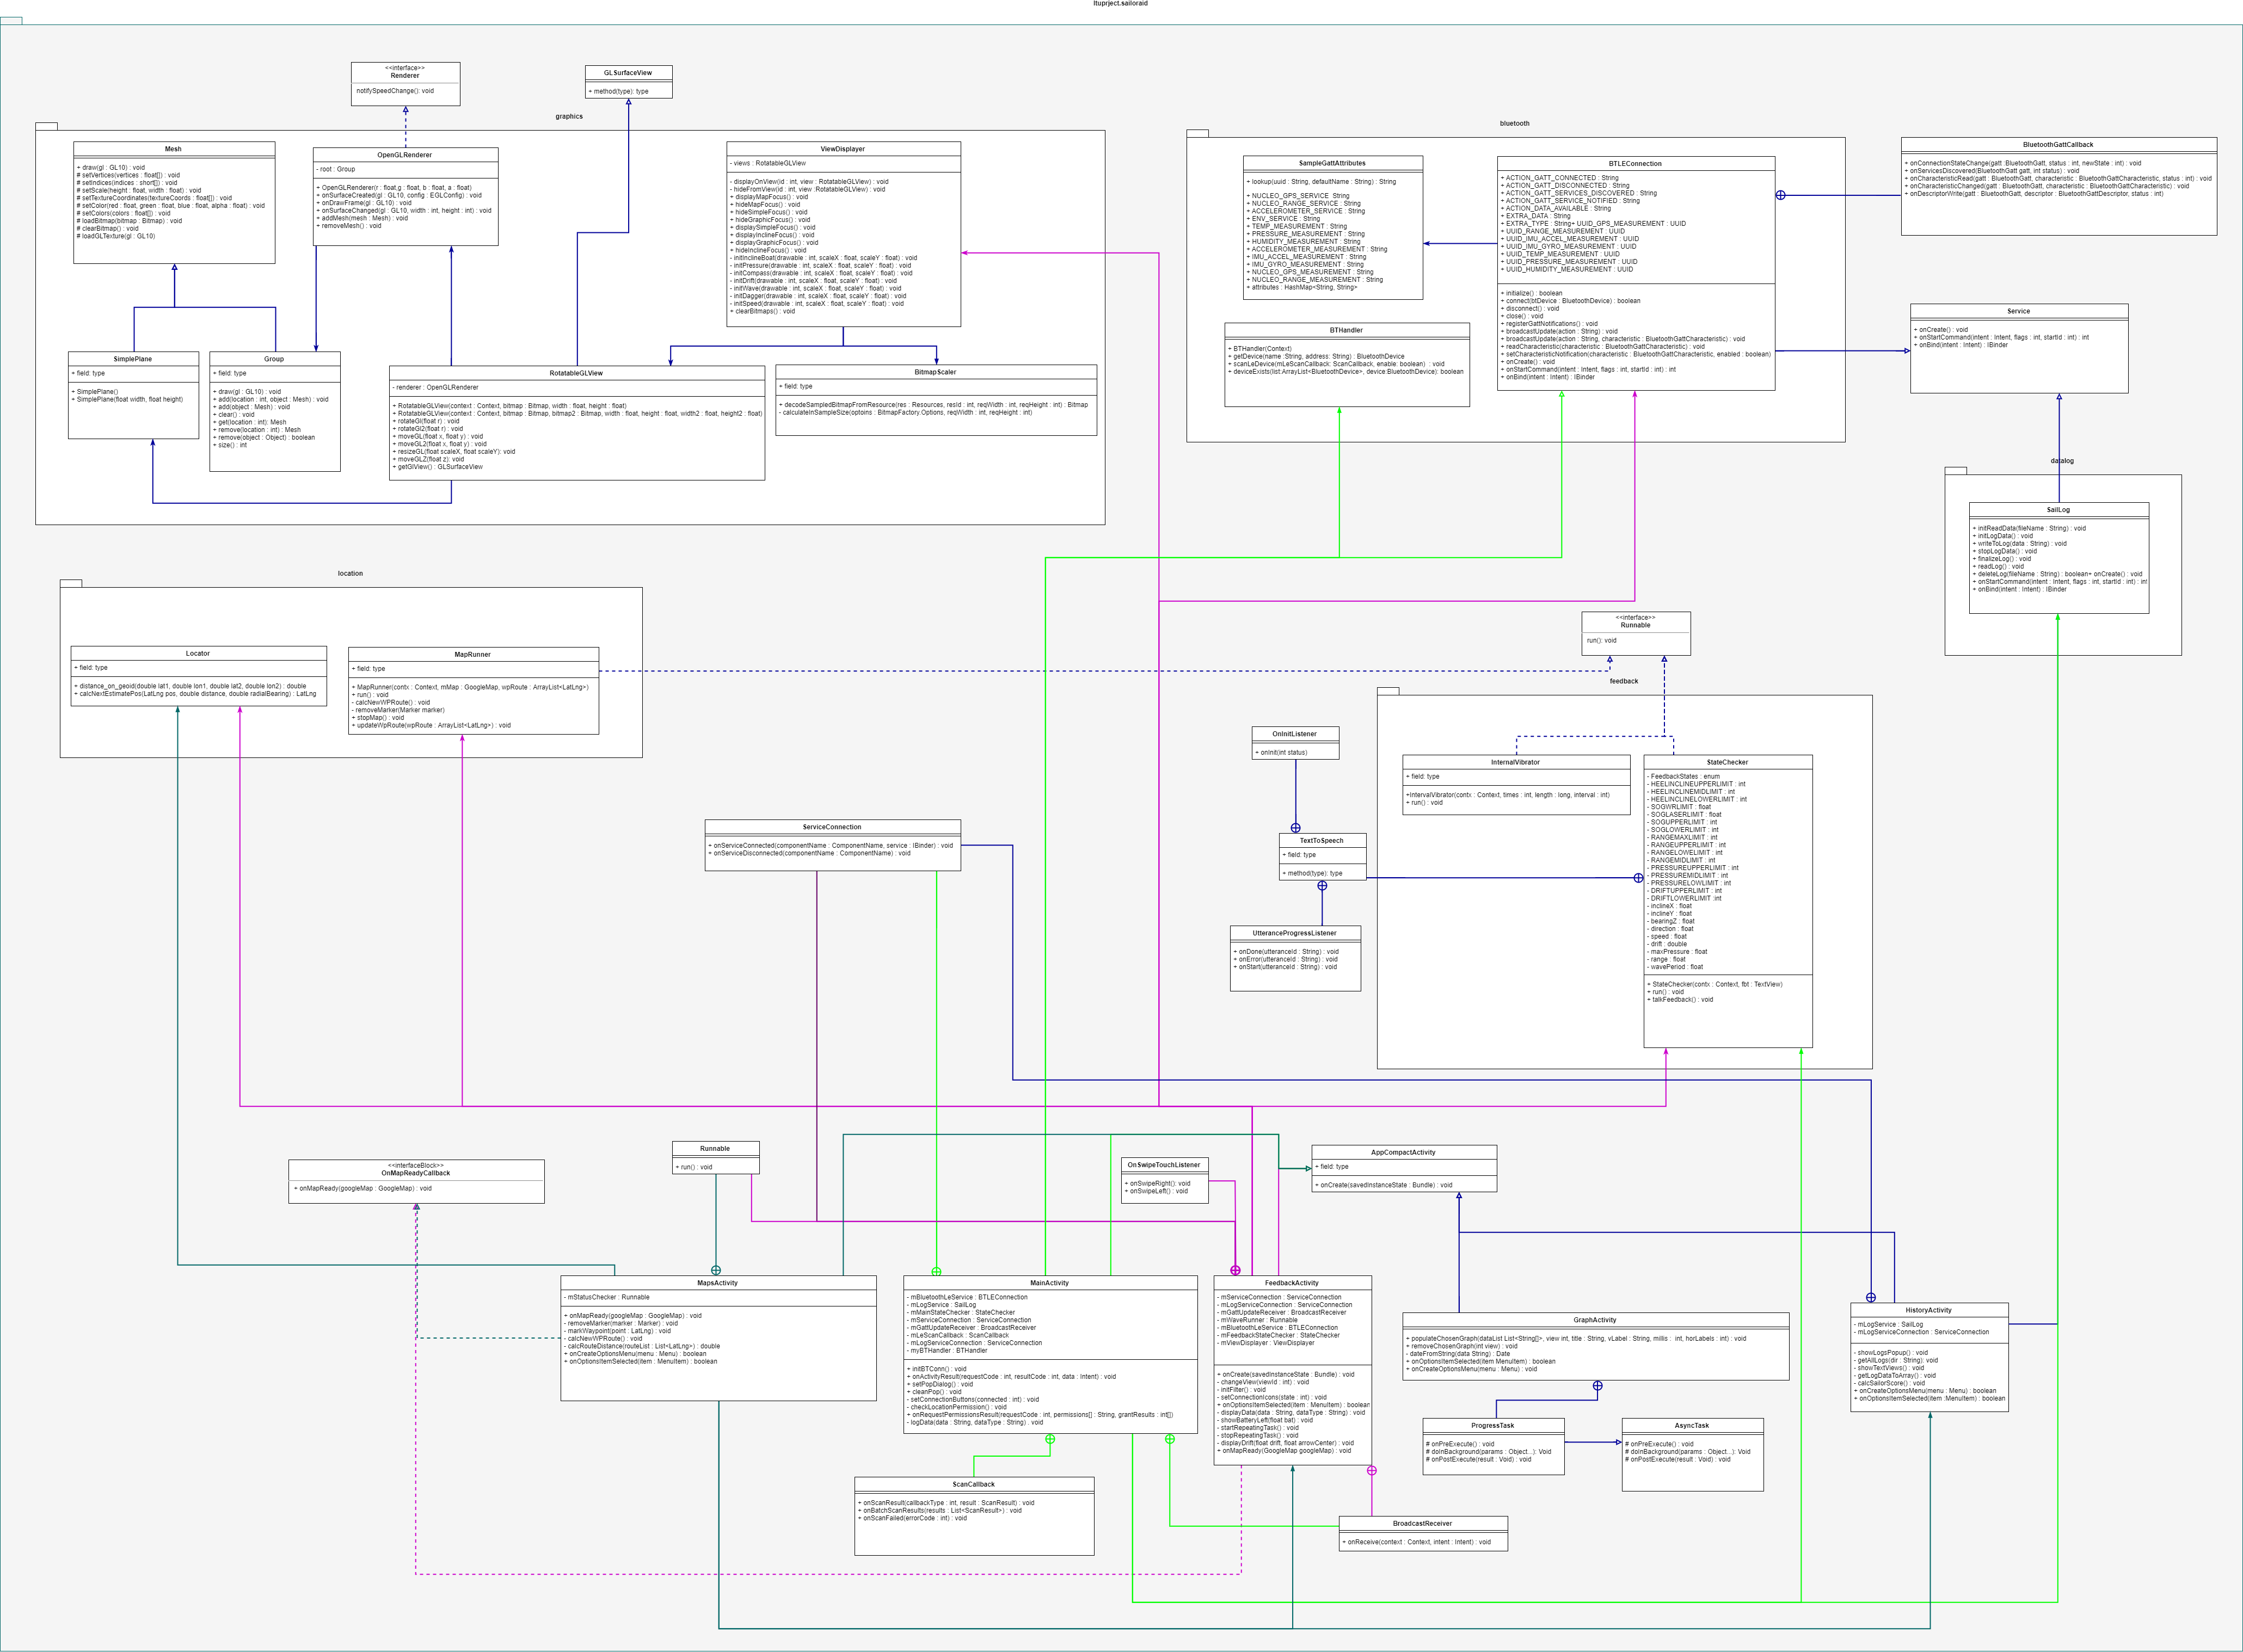
\includegraphics[width=1\textwidth]{Figures/uml.png}
\caption{UML model}
\label{android-uml}
\end{figure}
\begin{figure}[H]
\centering
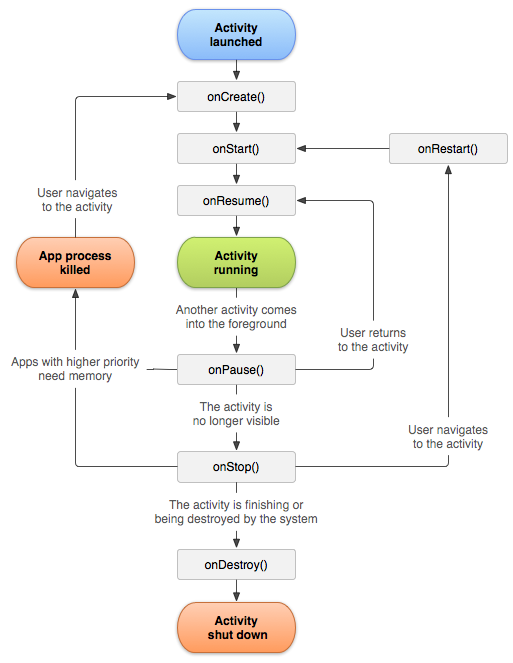
\includegraphics[width=0.8\textwidth]{Figures/activity_lifecycle.png}
\caption{Activity lifecycle}
\label{android-activity}
\end{figure}
The Bluetooth connection and data logging class is implemented as a services\cite{android-service}.A service could be started by an activity and continue running until it was explicitly called to stop. This allows several activities to share resources
and perform long-running operations in the background. The lifecycle
of a service was seen in Fig. \ref{android-service}.

\begin{figure}[H]
\centering
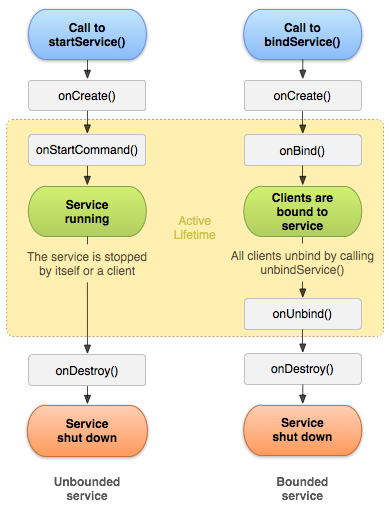
\includegraphics[width=0.8\textwidth]{Figures/service_lifecycle.png}
\caption{Activity lifecycle}
\label{android-service}
\end{figure}
\subsubsection{Feedback}
For the feedback states in the application, there are some approximations, and simplifications made for easier implementation. As explained in the Physics of sailing chapter there are certain parameters that can be evaluated in different states of the dinghy. An extensive approximation was that there is no water movement in the implementations. The states implemented are
\begin{labeling}{alligator}
\item [Clear] - The dinghy holds good velocity and not heeling or drifting and with a good amount of pressure on the ceneterboard
\item [Drift] - The dinghy is drifting perpendicular to the bearing while the centerboard is in an upper position
\item [Heel] - The dinghy has high heel angle
\item [Reefing] - The dinghy has high heel angle and the pressure on the centerboard is high
\item [Wrspeed] - The dinghys speed is above $65.45$kn
\item [Lrspeed] - The dinghys speed is above $16.8$kn
\item [Hike] - The dinghy has more then moderate heel angle and the pressure on the centerboard is between medium and high
\item [Keelhaul] - The dinghy has an above moderate heel angle and the centerboard is not in the lowest position
\item [Runninghigh] - The dinghy is sailing directly windwards with centerboard high and low heel angle.
\item [Runninglow] - The dinghy is sailing directly windwards with centerboard high and mid heel angle.
\item [Landcrab] - The dinghys speed is low.
\end{labeling}
Given these states, appropriate feedback could then be provided to the user. For handling states, a class called StateChecker was implemented. This would store sensor values and check against limits defined at an interval that was also defined in the class. Depending on these states this class would also determine what feedback that should be given.

\subsubsection{Visual Feedback}
It was determined that the visual feedback provided to the user was to include very little text information and would consist mainly of figures that changed position based on sensor data to give a good representation of what was going on with the dinghy. Because of different personal preferences, the ability to switch between different layouts was implemented. This was done by a simple swipe on the screen to toggle the view to the next layout. All layouts consisted of a subset of views from the complete set including
\begin{labeling}{alligator}
\item [\ref{feedback-incline} \textbf{Incline}]  displayed a ships relative incline against and artificial horizont.
\item [\ref{feedback-pressure} \textbf{Pressure}] moved a pin along a colored bar to represent high of low pressure applied on the centerboard.
\item [\ref{feedback-compass} \textbf{Bearing}] rotated a compass to show the ship relative bearing against true north.
\item [\ref{feedback-map} \textbf{Map}] displayed current location of the ship.
\item [\ref{feedback-drift} \textbf{Drift}] was represented with a colored bar with two arrows that moved to the relative drift direction to show the sailor if the ship was holding it's set navigaitional reference.
\item [\ref{feedback-height} \textbf{Speed}] displayed a speedometer from a classical Swedish vehicle\cite{volvo} with a movable bar representing speed over ground.
\item [\ref{feedback-sog} \textbf{Height}] of the centerboard was represented with a visual centerboard moving up and down along a graphical ruler.
\item [\ref{feedback-wave} \textbf{Wave frequency}] displayed a wave moving towards a ship at a speed representing different periods of the waves.
\item [\ref{feedback-text} \textbf{Feedback}] a text that changed values based on the current state of the boat.
\end{labeling}

\begin{figure}[H]
\centering
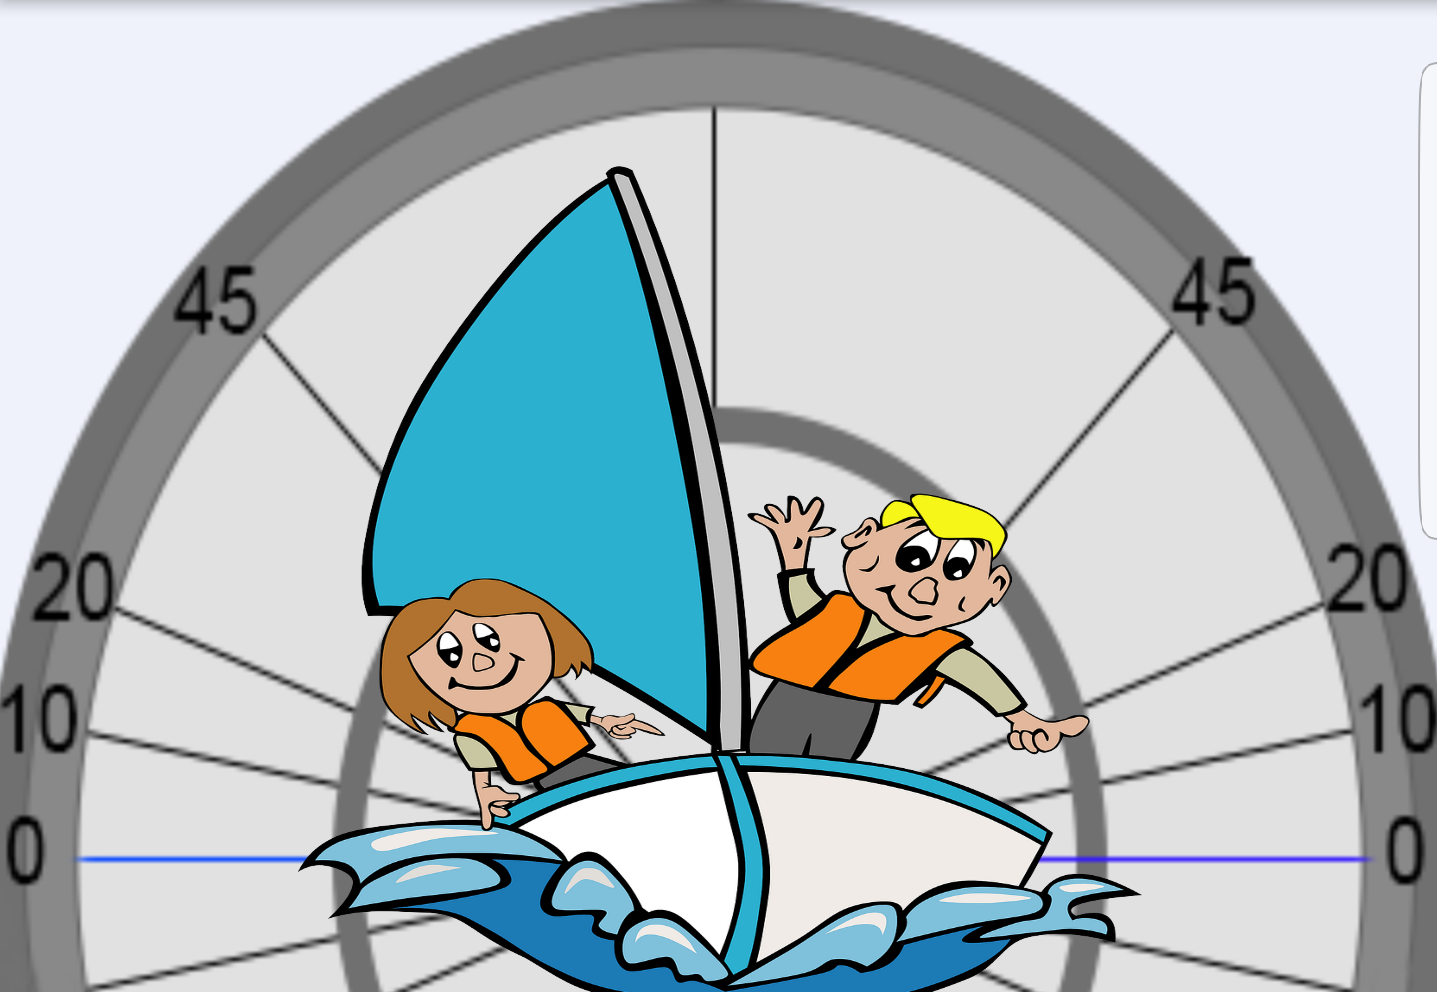
\includegraphics[width=0.6\textwidth]{Figures/incline.png}
\caption{Incline feedback view}
\label{feedback-incline}
\end{figure}
\begin{figure}[H]
\centering
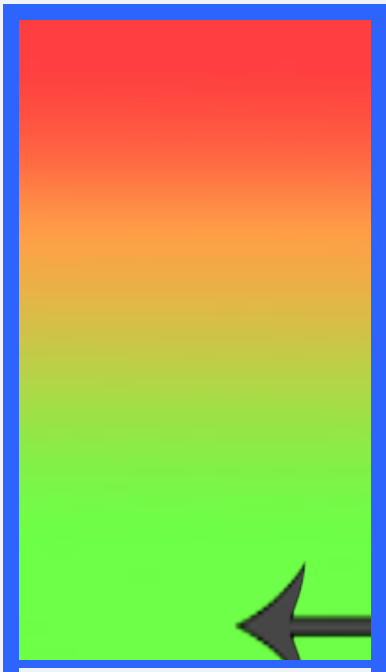
\includegraphics[width=0.3\textwidth]{Figures/pressure.png}
\caption{Pressure feedback view}
\label{feedback-pressure}
\end{figure}
\begin{figure}[H]
\centering
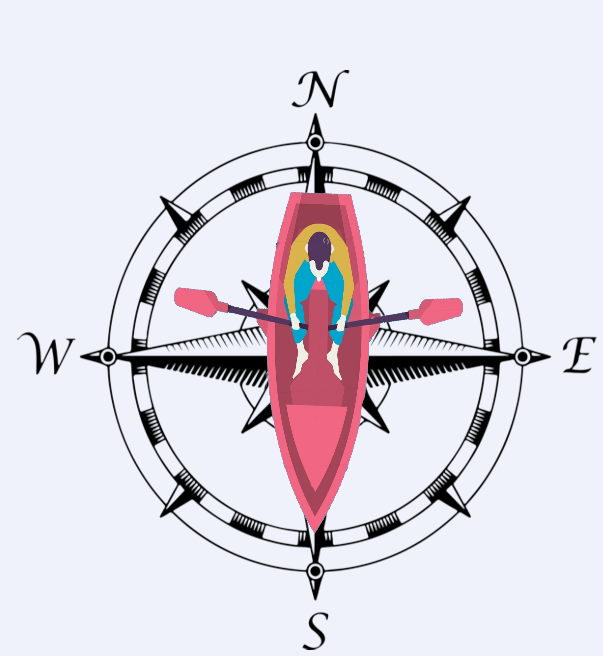
\includegraphics[width=0.6\textwidth]{Figures/compass.png}
\caption{Bearing feedback view}
\label{feedback-compass}
\end{figure}
\begin{figure}[H]
\centering
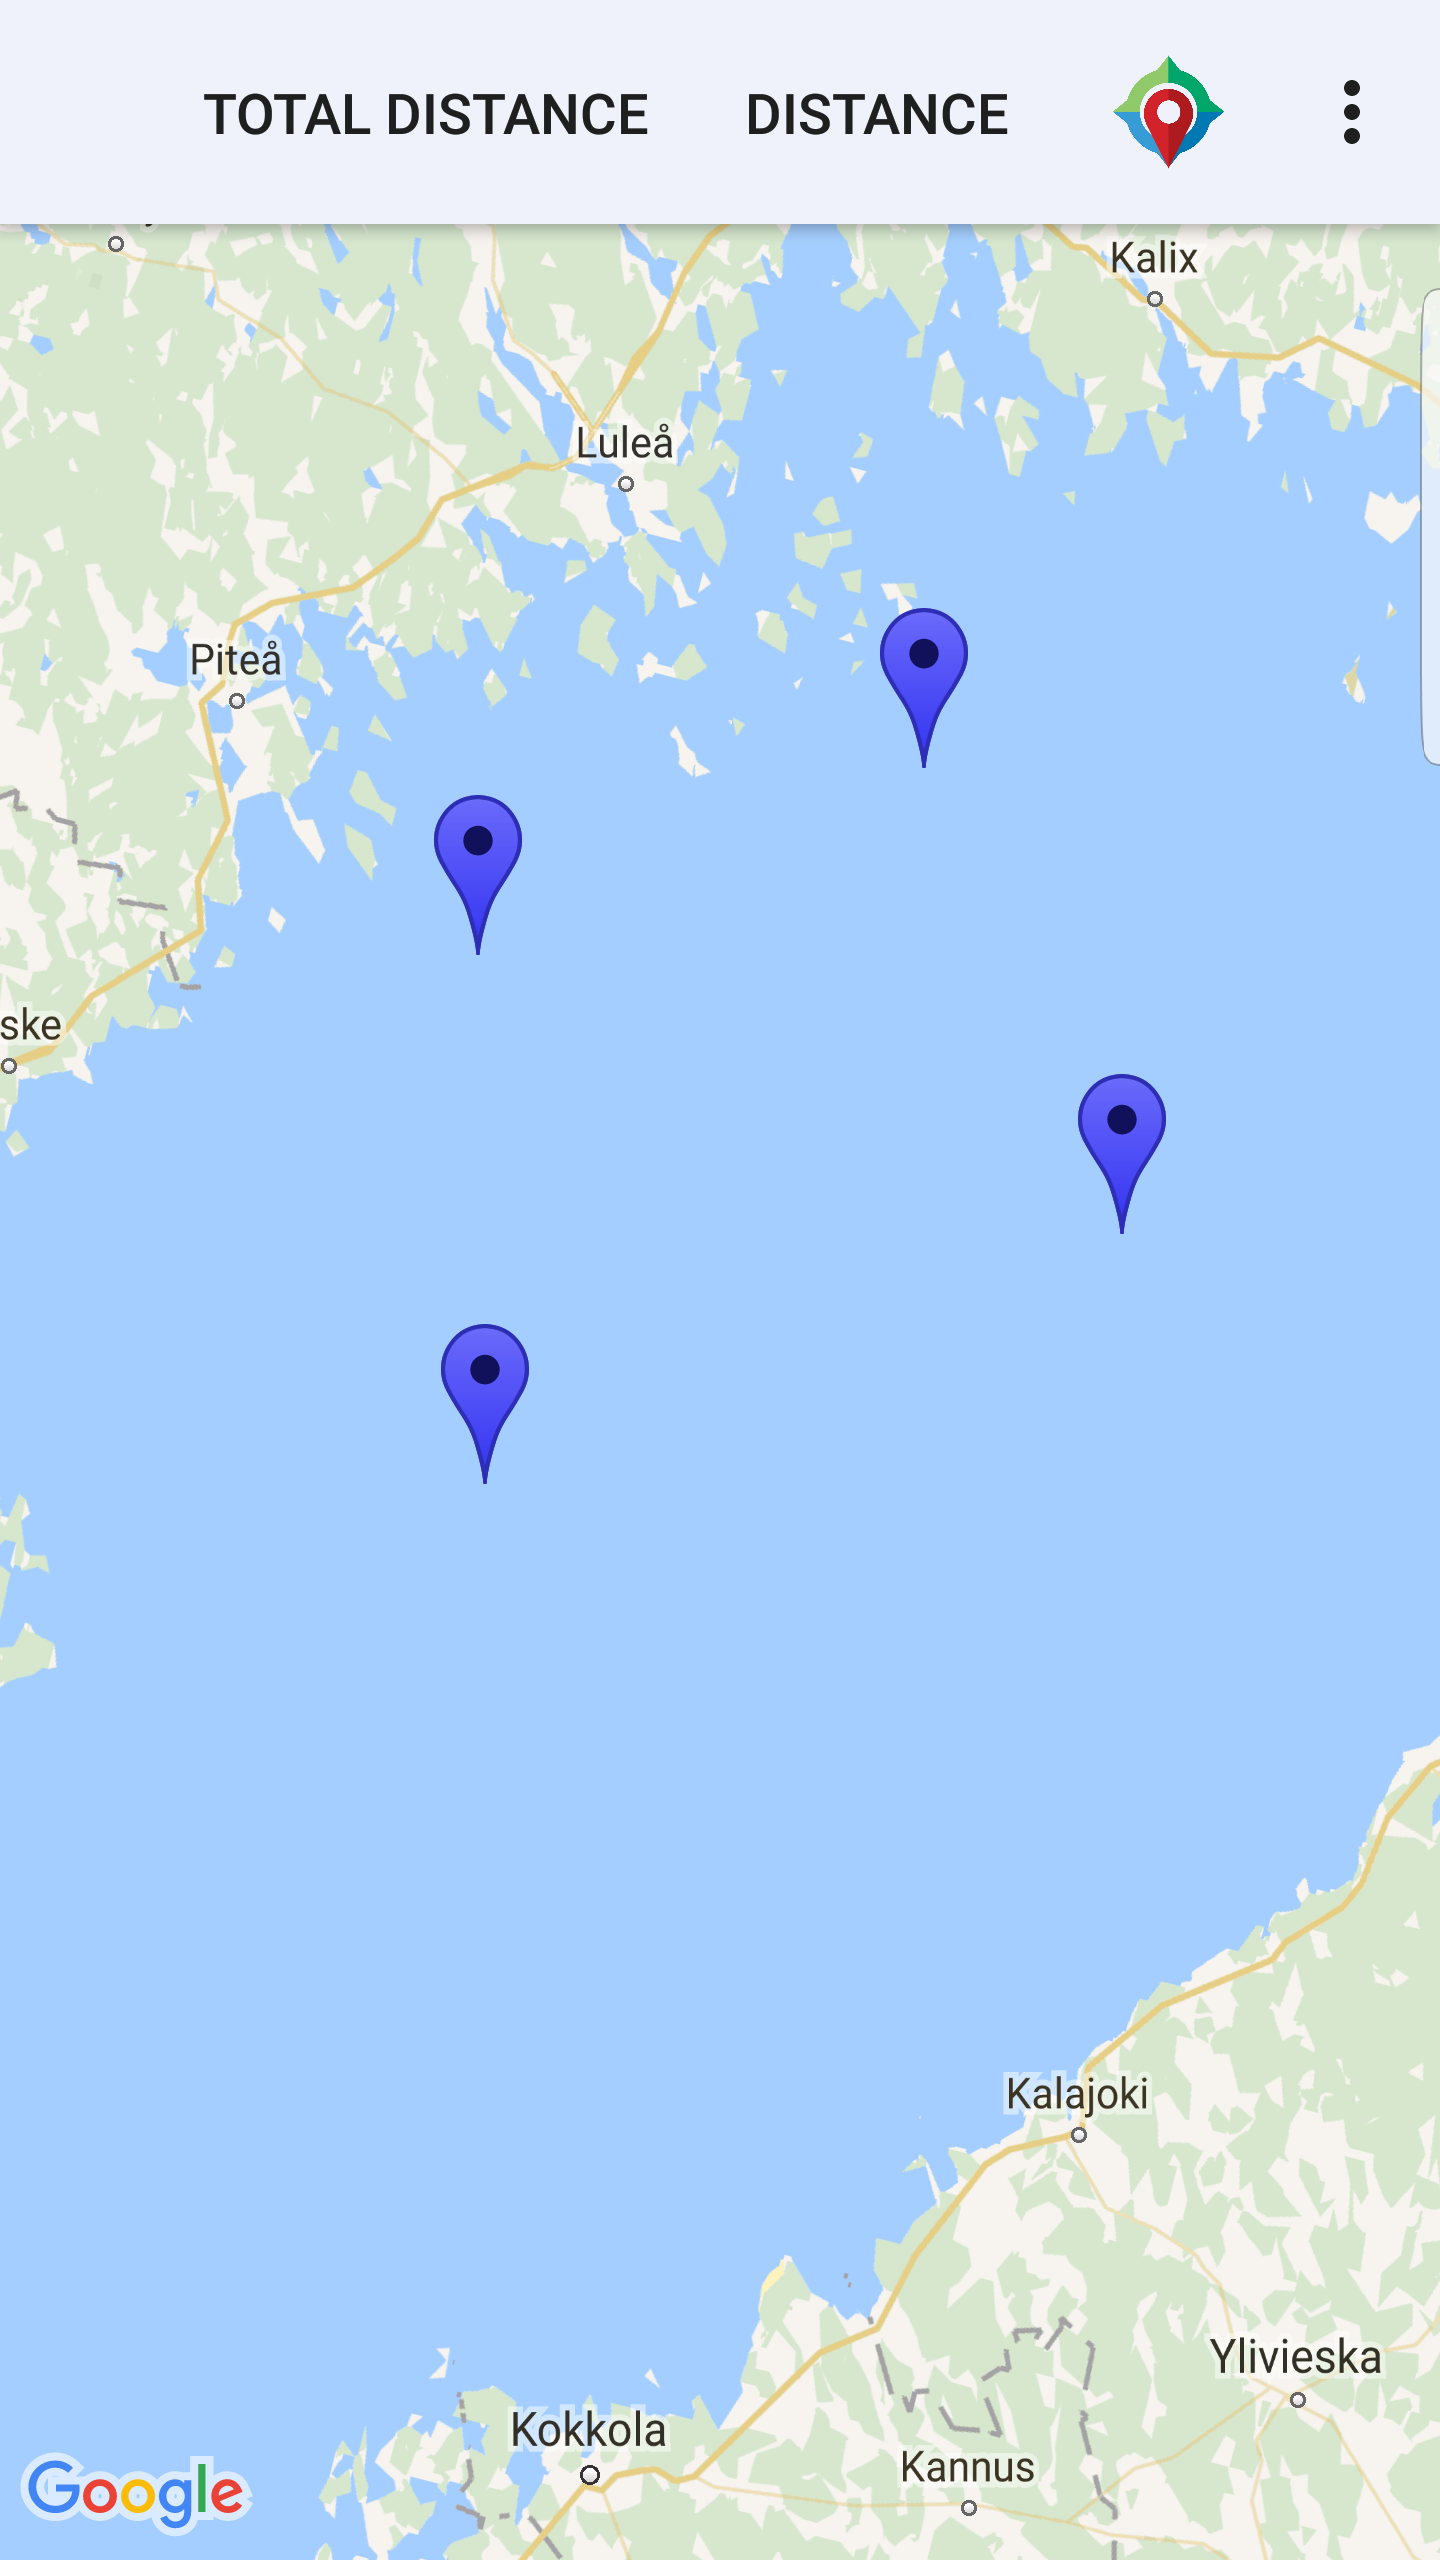
\includegraphics[width=0.4\textwidth]{Figures/map.png}
\caption{Map feedback view}
\label{feedback-map}
\end{figure}
\begin{figure}[H]
\centering
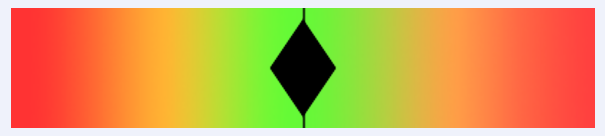
\includegraphics[width=0.6\textwidth]{Figures/drift.png}
\caption{Drift feedback view}
\label{feedback-drift}
\end{figure}
\begin{figure}[H]
\centering
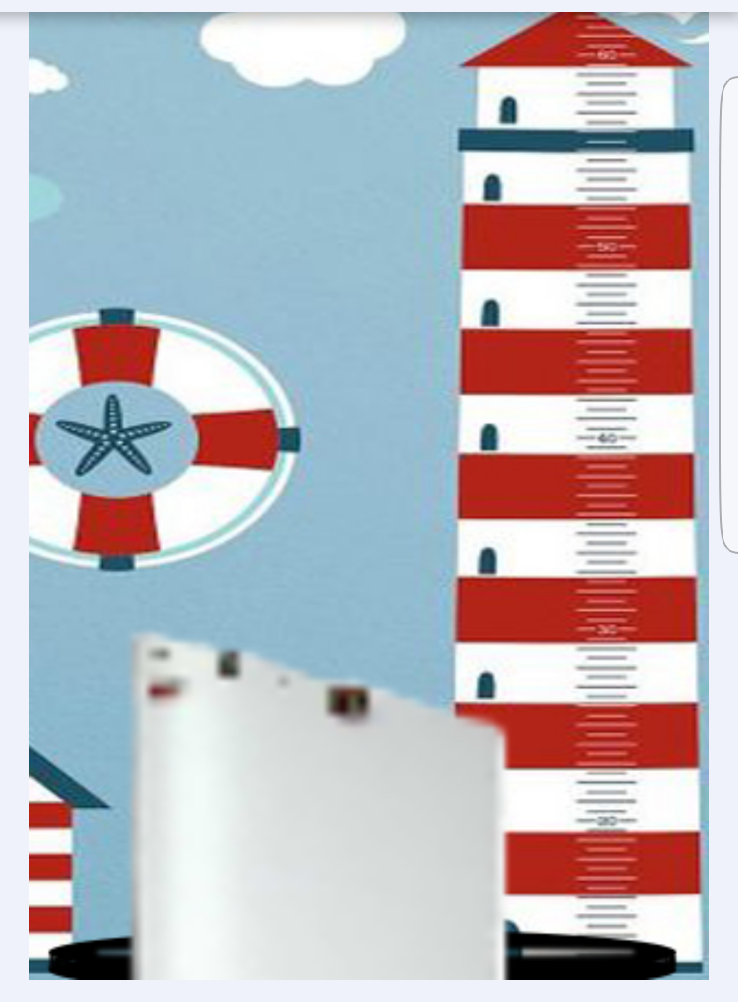
\includegraphics[width=0.4\textwidth]{Figures/height.png}
\caption{Centerboard height view}
\label{feedback-height}
\end{figure}
\begin{figure}[H]
\centering
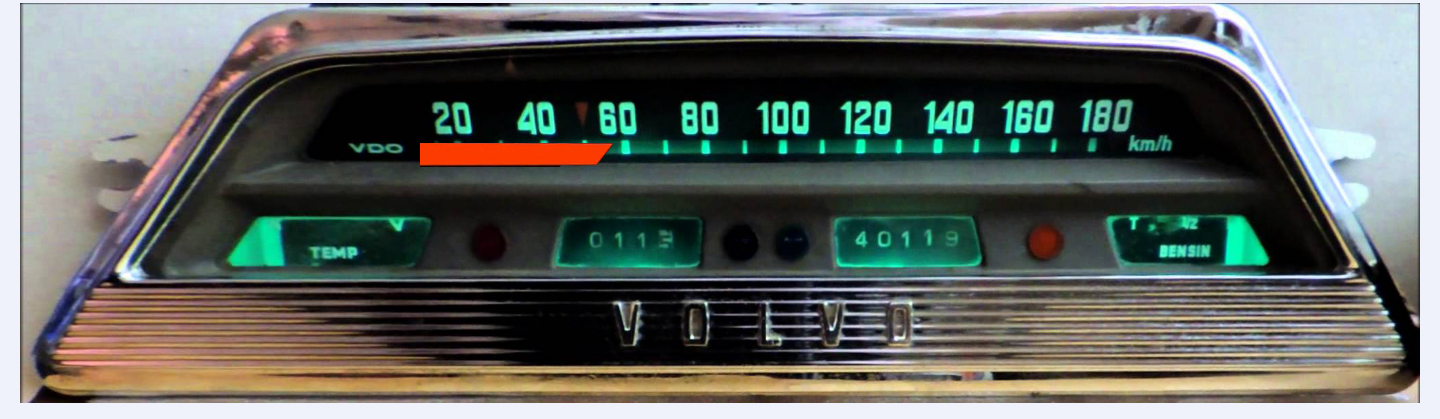
\includegraphics[width=0.8\textwidth]{Figures/sog.png}
\caption{Speed over ground view}
\label{feedback-sog}
\end{figure}
\begin{figure}[H]
\centering

\includegraphics[width=0.8\textwidth]{Figures/wave.png}
\caption{Wave period feedback view}
\label{feedback-wave}
\end{figure}
\begin{figure}[H]
\centering

\includegraphics[width=0.8\textwidth]{Figures/text.png}
\caption{Text feedback view}
\label{feedback-text}
\end{figure}
The figures were chosen at a development stage and improvements can easily be made by adding different \textit{PNG}\cite{png} files in android studio. They were implemented as GLSurfaceView\cite{gl} so that updating the figures could be done by calling a requestRender function, this improved the performance of the application when only updates to the figures were done when new sensor readings were received. To make the figure fit the application the GLSurfaceView was extended into a RotatableGLView that had the wanted features for rotation and positioning. Using these figures four different layouts were developed to give multiple choices for the user and was seen in figure \ref{feedback-layouts}. Switching between these layouts a swipeTouchListener was implemented which allowed the user to swipe across the screen to change the layout. Changing view the figures needed to be redrawn onto a new view matching the current layout, this was handled in the ViewDisplayer class that contained all RotatableGLViews.

\begin{figure}[H]
\centering
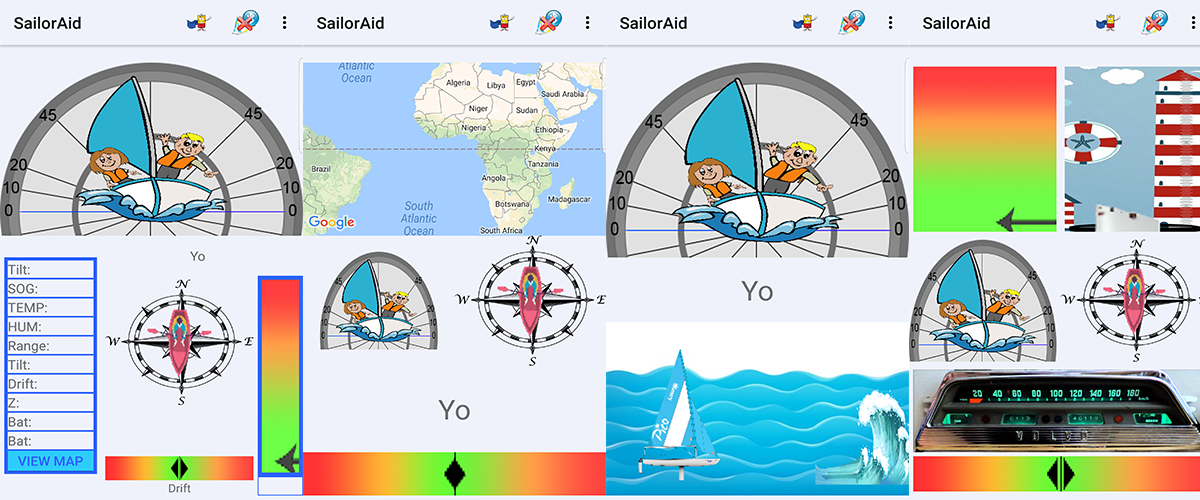
\includegraphics[width=0.8\textwidth]{Figures/layouts.png}
\caption{Different layouts}
\label{feedback-layouts}
\end{figure}

\subsubsection{Audio feedback}
Based on values from the sensors, different states were implemented and for each state, a text was read out to the user. The feedback was implemented such that the audio feedback would continue even if the device was put into sleep mode. Handling the text to speech feature a TextToSpeech\ref{texttospeech} class was implemented as an inner class in StateChecker. To prevent the speech to be interrupted preemptively an UtteranceProgressListener\cite{utter} was used. 

\subsubsection{Haptic feedback}
Based on the same states as the audio feedback vibration was also implemented. The frequency and length of the vibrations were implemented in such a way each state had a unique signature that could be recognized by the sailor after some practice with the system. Handling the interval a IntervalVibrator was implemented and run by the StateChecker.

\subsubsection{Log}
The ability to analyze the sailing trip was determined to be an important feature for the user, so a logging function was implemented so data could be stored in the device internal storage. This was handled by the SailLog class and these files could be read or deleted at a later stage, by the user. Storing a log was implemented such that the sailor would need to start a logging session after Bluetooth connection had been established to the ship. After the log was started it would create a file on the device internal storage and write sensor data to the file at the same frequency as the data was transmitted by the system. While logging was active the device would continue to store information even if the device was put in sleep mode so that the sailor could choose to only log data and not view the information displayed on the screen. After the sailing trip was finished the sailor could read the saved log file and receive a summary of the trip (Fig. \ref{log-summary}). More information from the log could be analyzed by reading graphs (Fig. \ref{log-graph}) where the sensor data was shown with respect to time. These graphs were implemented such that the user was able to choose what graphs to be displayed on the device for improved comparability.
\begin{figure}[H]
\centering
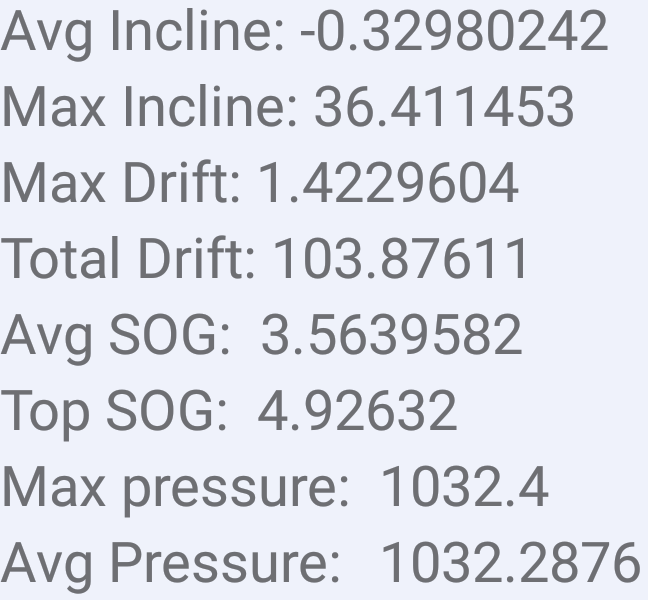
\includegraphics[width=0.4\textwidth]{Figures/log_data.png}
\caption{Log data summary}
\label{log-summary}
\end{figure}
\begin{figure}[H]
\centering
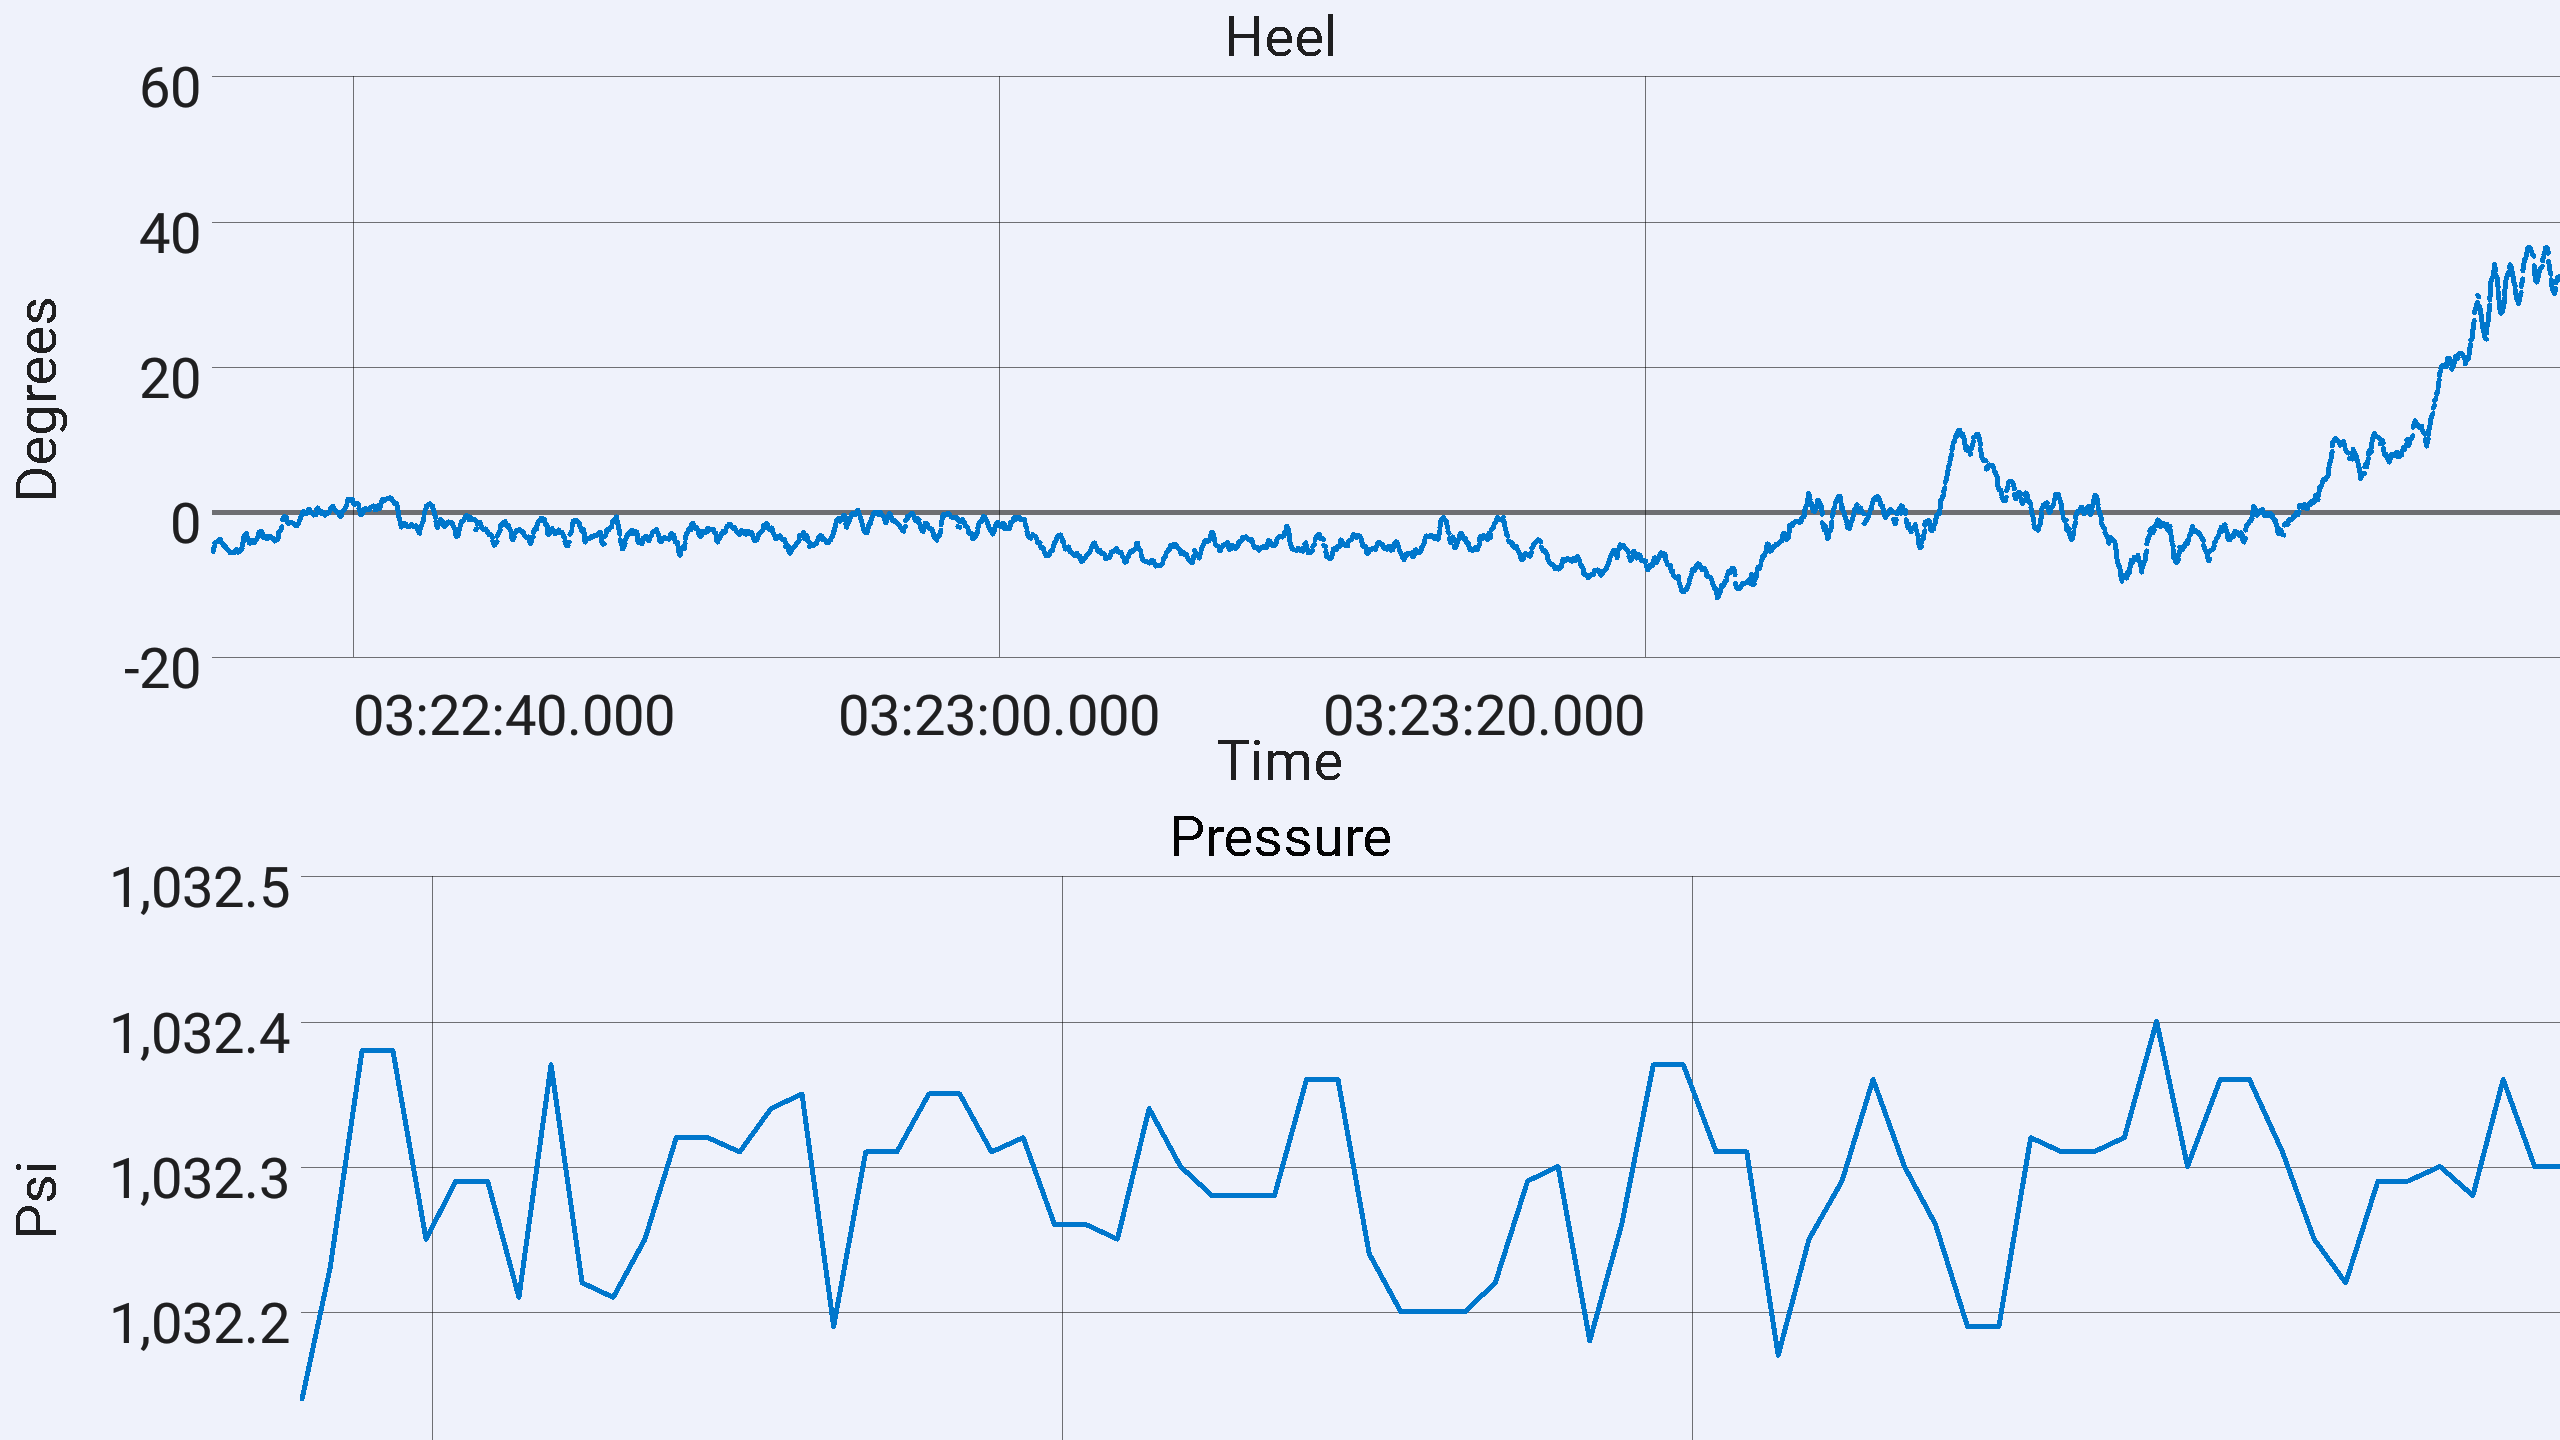
\includegraphics[width=0.7\textwidth]{Figures/log_graph.png}
\caption{Log graphs}
\label{log-graph}
\end{figure}

\subsubsection{Bluethooth connection}
A list of all devices in the nearby area was displayed when the user decided to connect to the system, this added flexibility to the user and allowed connection between multiple systems with different MAC-addresses. Scanning for nearby devices was done in the MainAcivity and handled by the BTHandler class. The application uses Bluetooth low energy technology to match the systems implementation. This allowed the device to receive notifications when the data is altered on the system and updates would occur in different frequencies for different types of data. To ensure a stable connection between the system and the device the connection class was implemented as an android service\cite{android-service}. This allowed the device to keep the connection alive between different views and even when the device was put into sleep mode. All functionality regarding connecting and receiving data was implemented in the BTLEConnection class and known characteristics and the determined unique Gatt service identifiers were stored in the SampleGattAttributes class.

\subsubsection{Map}
For the sailor to get more information about location two maps were implemented, one that was embedded into a layout in the FeedbackActivity and the functionality of this was handled in the MapRunner class, the other map was implemented in MapsActivity. This could be improved by using the same class for both maps to achieve better readability and modifiability of the code. Both these implementations utilized the Google maps API\cite{gmaps}, which could be used freely and the map service is highly accurate and suited our system well. Interaction with the maps could also be made quite easily which helped to make development faster. The sailor had the ability to see a path over the trip and the total distance traveled. Waypoint could be placed if the sailor wanted to decide in advance a certain trip. The distance of all the waypoints was displayed and the distance currently traveled to give the sailor information on how long the trip was and how much of the trip was left to be sailed. A path to the nearest waypoint was shown to help navigation when the sailor was close to the first waypoint the path to the next waypoint was shown. The waypoint route could also be viewed in the map of the FeedbackActivity layout.

\subsubsection{Drift}
Calculation of leeward drift was done by inspection the distance from an estimated destination point and the position received from the \textit{GPS}. By using the \textit{GPS} position and the ships bearing from the systems magnetometer a \textit{rhumb line}\cite{rhumb-line} was derived and the new estimated position was calculated with
%δ = d/R	(angular distance)
%φ2 = φ1 + δ ⋅ cos θ	
%Δψ = ln( tan(π/4 + φ2/2) / tan(π/4 + φ1/2) )	(‘projected’ latitude difference)
%q = Δφ/Δψ (or cos φ for E-W line)	
%Δλ = δ ⋅ sin θ / q	
%λ2 = λ1 + Δλ
\begin{align*}
  &\begin{aligned}
  \delta &= d/R 
  \end{aligned}\\
 &\begin{aligned}
  \varphi_2 &= \varphi_1 + \delta \cdot \cos{\theta}
  \end{aligned}\\
 &\begin{aligned}
  \Delta\psi = \ln { \bigg( \tan{\frac{n}{4} + \frac{\varphi_2}{2}} \bigg/ \tan{\frac{n}{4} + \frac{\varphi_1}{2}} \bigg)}
  \end{aligned}\\
 &\begin{aligned}
  q = \frac{\Delta\varphi}{\Delta\varphi}
  \end{aligned}\\
 &\begin{aligned}
  \Delta\lambda = \delta\cdot\sin\frac{\theta}{q}
  \end{aligned}\\
 &\begin{aligned}
  \lambda_2 = \Delta\lambda_1 + \Delta\lambda
  \end{aligned}\\
\end{align*}
where $R$ is the Earth's radius, $d$ is the distance traveled, $\theta$ is ships bearing, $\lambda_1$ and $\varphi_1$ is the point of origin in longitude and latitude. This new estimated position $\lambda_2$ and $\varphi_2$ was then compared to the next positional data from the \textit{GPS} and the distance between these points was calculated using \textit{Equirectangular projection}\cite{equirectangular}
%x = Δλ ⋅ cos φm
%y = Δφ
%d = R ⋅ √x² + y²
\begin{align*}
  &\begin{aligned}
  x = \Delta\lambda \cdot \cos\frac{\Delta\varphi}{2}
  \end{aligned}\\
 &\begin{aligned}
  y = \Delta\varphi
  \end{aligned}\\
 &\begin{aligned}
  d = R\cdot\sqrt{x^2+y^2}
  \end{aligned}\\
\end{align*}
where $\Delta\lambda$ and $\Delta\varphi$ are the differences in longitude and latitude for two location points. This function had high performance gain but was less accurate over large distances then, e.g., the \textit{Haversine formula}\cite{haversine}. Since for this function, only small changes in distance were calculated the accuracy was more than adequate. A problem with this way of calculating leeward drift is the accuracy of the \textit{GPS} readings and to get a good bearing the idea was to make use of the magnetometer though the accuracy of that is also far from perfect and a small deviation of a couple of degrees resulted in a large drift. The solution was to use the directional data sent from the GPS module which calculates direction based on last positional data. This solution would work well for progress in the forward direction and when fast sideways motion is detected the estimated position would be along the same vector as the previous direction. However, for constant drift sideways this approach would display that no drift was taking place. This calculation was handled by the Locator class.

























